%\documentclass[a4paper,openright,12pt]{book}
%
%\usepackage[utf8]{inputenc}
%\usepackage[spanish]{babel}
%\usepackage{amsmath}
%\usepackage{fancyhdr}
%\usepackage{todonotes}
%\usepackage{graphicx}
%\usepackage{float}
%% aqui definimos el encabezado de las paginas pares e impares.
%%\lhead[Daniel Albendín y ángel Cantó]{Daniel Albendín y ángel Cantó}
%%\chead[]{}
%%\rhead[Resumen]{Resumen}
%%\renewcommand{\headrulewidth}{0.5pt}
%%
%%% aqui definimos el pie de pagina de las paginas pares e impares.
%%\lfoot[Universidad de Huelva]{Universidad de Huelva}
%%\cfoot[\thepage]{\thepage}
%%\rfoot[Proyecto Semandal]{Proyecto Semandal}
%%\renewcommand{\footrulewidth}{0.5pt}
%
%
%
%% Este es un comentario, no será mostrado en el documento final.
%\begin{document}

\chapter{Obtención de municipios y sus datos}
\label{chap:obdat}
Nuestro proyecto gira en torno a los municipios y queríamos integrar información de estos desde distintas fuentes. Para ello lo que necesitábamos era una lista oficial de municipios y encontramos un \textit{CSV} con todos los municipios españoles a día \textbf{01/01/2014} con algunos datos. Con este fichero empezamos a importar los datos a nuestra base de datos para tener la tabla con todos los pueblos para poder realizar búsqueda de otros datos que explicaremos posteriormente. El fichero en cuestión era el \textbf{CODMUN14.xls} \href{www.ine.es/daco/daco42/codmun/codmun14/14codmun.xls}{www.ine.es/daco/daco42/codmun/codmun14/14codmun.xls} 
, pero como podemos comprobar los datos de este pueblo son bastante escasos, así que tuvimos que buscar más datos de todos los pueblos españoles. Consultamos la página del INE (Instituto Nacional de Estadística) y encontramos un fichero con la deuda de todos los municipios españoles a fecha \textbf{31/12/2013} e incorporamos los datos. También encontramos un fichero con los habitantes, y la superficie, etc \ldots 

En una primera aproximación, decidimos que íbamos a centrarnos en realizar una extracción de datos desde las páginas web de los ayuntamientos, por tanto faltaban datos necesarios para nosotros que no estaban en los xls citados anteriormente cómo la url de la página web de cada pueblo, el más importante ya que sin este no podríamos obtener la información accesible únicamente desde éstas, las coordenadas y la página de wikipedia.

Como posible implementación extra, decidimos usar un listado de provincias españolas, para poder tener a que provincia pertenece un municipio. Para la APP esta información no sirve de mucho, (únicamente para decir en que provincia está un pueblo) pero desde la API se puede llegar a consultar los pueblos de una provincia, y sus correspondientes datos.

Para la obtención de estos datos, usaremos varias APIs de Google y realizaremos varios scripts que funcionaran como wrappers.
A continuación explicaremos es funcionamiento del estos scripts.

\section{Obtención de pueblos y datos a partir de xls}
	Como explicamos en la introducción, el listado de pueblos y algunos datos lo obtenemos de tres xls. Por tanto debemos realizar parseadores de xls para obtener los datos y llevarlos a la base de datos por lo que debemos tener creadas las tablas en ésta y a partir de ahí podemos empezar a crear registros o actualizarlos. 
	
La extracción de datos no se hizo de forma incremental empezando por los xls y posteriormente los datos extraidos con scripts de internet, si no que creamos la tabla y fueron surgiendo propuestas de atributos para los municipios almacenados, por tanto tuvimos que cambiar en varias ocasiones la estructura de la base de datos.

Cuando creamos la base de datos en primer lugar, se guardaron los nombres de los pueblos y se asoció una correspondiente ID a cada uno. Ese ID no venía en los distintos documentos así que tuvimos que hacer una búsqueda por el nombre del pueblo, en nuestra tabla de datos y actualizar los valores necesarios. Para esto un municipio debería llamarse igual en los tres archivos xls que teníamos y al ser documentos oficiales este hecho se constata y hemos unificado los datos de los distintos xml en nuestra base de datos.

\section{Extracción de url de los ayuntamientos}

La extracción de las direcciones web de los ayuntamientos ha sido posible gracias a la API de búsqueda de Google, \textit{Custom Search}, que nos permite realizar 100 búsquedas con el motor de búsqueda de Google pudiendo modificar éste con ciertos parámetros que la \textit{Custom Search} nos permite cambiar como por ejemplo el idioma, la región o el número de respuestas que queríamos en una llamada (limitada a 10).

Creamos el buscador, y hacemos referencia al éste, con la id que nos da Google cuando lo creamos, en la url de la llamada a la API\textit{Custom Search}. Hemos usado como palabras claves el nombre del pueblo ayuntamiento y la comunidad autónoma, para evitar confusiones de dos pueblos con el mismo nombre.

El inconveniente de este método es el límite diario de búsquedas que te tiene. La respuesta de esta API es en formato JSON. En los resultados de esta API, podemos obtener datos no válidos para nuestra experimentación. En nuestro caso nos hemos encontrado con resultados en las respuestas JSON de páginas que no eran las del ayuntamiento (En ocasiones normales porque éste no tenía) como por ejemplo \textit{ayuntamiento.es} \href{http://www.ayuntamiento.es/}{http://www.ayuntamiento.es/}, \textit{páginas amarillas} \href{www.paginasamarillas.es/}{www.paginasamarillas.es/}, y otras páginas webs la cual nos daban información sobre los pueblos en lugar de la página del ayuntamiento como la página del ayuntamiento de badajoz. Y en ocasiones, si la llamada a la API nos daba 10 resultados, un 80\% de los enlaces devueltos por la búsqueda con nuestro motor, eran de este tipo.

Para la diferenciación de los pueblos que no tienen página web del ayuntamiento con los que no han sido explorados todavías, ponemos el campo url de los pueblos en la tabla de datos a null por defecto, y los pueblos que exploramos y no tienen página web del ayuntamiento lo marcamos como analizado.


Es importante mencionar que aunque este proyecto se centra en los pueblos andaluces, Y en concreto con OpenCMS, se han configurado varios buscadores, para abarcar también municipios que tienen otra lengua además del castellano ya que en dichos municipios la búsqueda tiene un mayor porcentaje de éxito si tienen la palabra \textbf{Ayuntamiento} en dicha lengua.

Tenemos más de 8000 municipios españoles, y tenemos las url de los ayuntamientos de un 50\% aproximadamente. La ejecución de este script debe ser un proceso supervisado y cuando decidimos acortar el número de pueblos con los que íbamos a trabajar, decidimos que únicamente íbamos a trabajar con municipios andaluces, optamos por dejar de actualizar las urls de los municipios y dejar el resto para trabajos futuros. 

Hay páginas webs de algunos ayuntamientos los cuales o han cambiado de dirección, o la página principal se encuentra en una url del mismo dominio pero no en el index, y éstas páginas con la etiqueta \textit{http-equiv=x\_refresh} 
redireccionan a la auténtica página principal del ayuntamiento.

La base teórica de este script se centra en la necesidad de estar en la página principal para navegar a través de ésta para realizar la recopilación de datos automáticamente.
Por eso aunque al usuario le damos la url tal y como la recuperamos del script sin redireccionar, ya que el usuario accederá a través de un navegador, para nuestro uso a la hora de realizar el scrap a los datos de los ayuntamientos, este script es necesario.
\begin{figure}
\centering
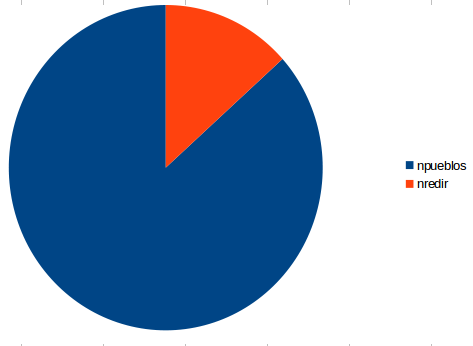
\includegraphics[scale=0.5]{./obdat/imagenes/redir.png}
\caption{Porcentaje de pueblos con redirección}
\label{redireccion}
\end{figure}

\section{Obtención de coordenadas}

Para la obtención de coordenadas hemos usado la API de Geolocalización de goolge ( \textit{Geocode}). Para la construcción de la búsqueda en la API, usamos la estructura de \textbf{pueblo + provincia + españa} (Para evitar confusión).

La respuesta de la API es en JSON, así que accediendo a las posiciones adecuadas de los arrays devueltos, podemos obtener la latitud y la longitud de nuestros municipios.

hemos construido un fichero \textbf{plantilla\_vacia.html} con el contenido necesario para mostrar un mapa de Google maps en blanco, sin ningún tipo de marcador. Este fichero necesita una API key, única para cada usuario, que nos permite visualizar el mapa. Una vez creado este fichero, obtenemos la latitud y longitud de todos nuestros municipios en un script que se encargará de, a nuestro mapa en blanco, agregar los datos adecuados para representar los municipios que elijamos, como por ejemplo, mostrar los municipios de los que tenemos noticias almacenadas en la base de datos.

\begin{figure}
\centering
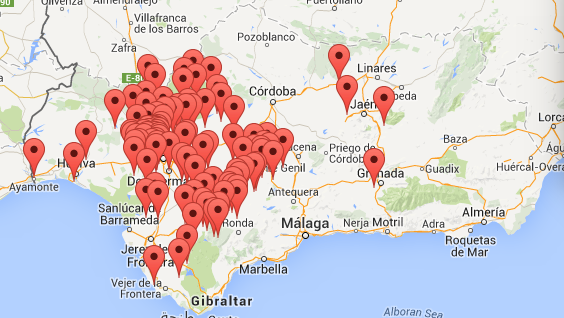
\includegraphics[scale=0.5]{./obdat/imagenes/p_noticias.png}
\caption{Pueblos con noticias en Semandal}
\label{fig:pueblos_noticias}
\end{figure}


A continuación mostramos todos los pueblos que tenemos (Ver figura \ref{fig:imagen_todos}) y una prueba de que el pueblo que nos muestra está correctamente posicionado (Ver figura \ref{fig:imagen_uno})

\begin{figure}
\centering
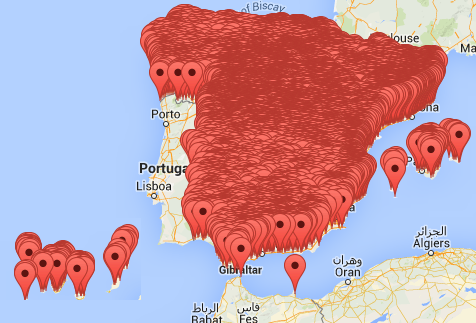
\includegraphics[scale=0.5]{./obdat/imagenes/Todos.png}
\caption{Pueblos de España}
\label{fig:imagen_todos}
\end{figure}

\begin{figure}
\centering
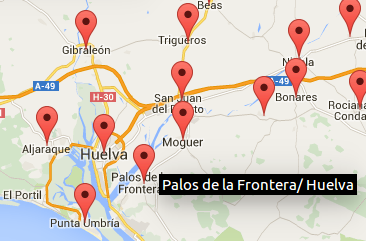
\includegraphics[scale=0.5]{./obdat/imagenes/NombresPueblos.png}
\caption{Prueba del correcto posicionamiento de los pueblos}
\label{fig:imagen_uno}
\end{figure}
\section{Búsqueda de municipios cercanos}

Una vez obtenidas todas las coordenadas de los distintos municipios decidimos determinar para cada municipio los cinco municipios más cercanos. Para hacer el calculo se determina la distancia de cada municipio con el resto, luego se ordena la lista generada de menor a mayor para tomar los cinco primeros, que son los cinco municipios más cercanos.

\section{Páginas con OpenCMS}

Al acotar el radio de actuación del proyecto a los pueblos que tenían OpenCMS o no, debíamos saber que pueblos implementaban esta opción. La dificultad que tiene este tipo de pueblos, es que algunos si tienen en su redirección el \textit{/opencms/opencms} pero otros aunque la página index.hml sea la misma que se encuentra en /opencms/opencms/index.html no lo redireccionan, por tanto hemos hecho un script que nos dice qué municipios tienen su página web funcionando bajo la plantilla opencms. Así a la hora de recopilar datos, con una consulta, nos traemos los pueblos que tienen el campo opencms marcado.


\begin{figure}
\centering
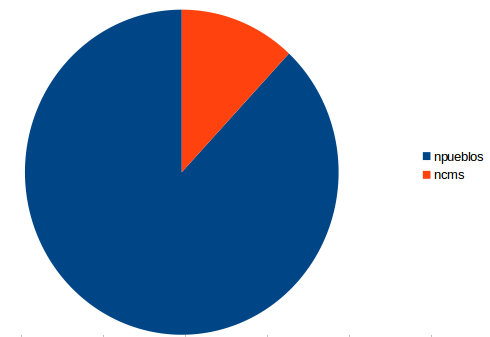
\includegraphics[scale=0.5]{./obdat/imagenes/cms.png}
\caption{Porcentaje de pueblos con OpenCMS}
\label{fig:openCMS}
\end{figure}

\section{Página de wikipedia}

A la hora de obtener la página de wikipedia, sólo queremos la página que tenga una bandera o escudo, para mostrarla en la aplicación. 

El problema a la hora de buscar pueblos es que en ocasiones nos podemos encontrar con una página de desambiguación, por este motivo debemos implementar dos scripts, uno que cuando no se encuentre la palabra desambiguación actualice la url de wikipedia del pueblo, y cuando se encuentre una página de desambiguación, use el mismo método que hemos usado para buscar las url de los pueblos, es decir la API \textit{Custom Search} de Google, buscando esta vez la palabra wikipedia más el nombre del municipio más la provincia.

Existe un caso específico en el que  este algoritmo falla y es cuando la búsqueda no nos da error o desambiguación, y la página que encontramos no es la del pueblo. De momento los casos que hemos encontrado son: LOJA, QUESADA, GALERA.



%\end{document}
